\chapter{Background}
\label{chp:background} 

\section{NetFlow}
Cisco IOS NetFlow creates an enviroment that have the tools to understand who, what, when, where and how network traffic is flowing. This makes it easier for administrators to utilize the network as optimal as possible. One can determine the source and destination of traffic and use this information to reveal for example DDoS-attacks or spam mail. 

\subsection{How dies it work?}
Every packet that is forwarded within a router/switch is examined for a set of IP packet attributes. With these attributes one can determine if the packet is unique or similar to other packets. 

The attributes used by NetFlow are:
\begin{itemize}
\item IP source address
\item IP destination address
\item Source port
\item Destination port
\item Layer 3 protocol type
\item Class of service
\item Router/Switch interface
\end{itemize}

To group packets into a flow, one compares source/destination IP address, source/destination ports, protocol interface and class of service. Then the packets and bytes are tallied. This method is scalable because a large amount of network information is condensed into a database of NetFlow information called the NetFlow cache. 

When the NetFlow cache is created one can use this to understand the network behaviour. The different attributes generate different knowledge about a certain network, and combined they can paint a detailed picture of how the network is working. For example the ports show what application is utlizing the traffic, while the tallied packets and bytes show the amount of traffic. 

\todo{Lime inn hvordan det ser ut i kommandolinjen}

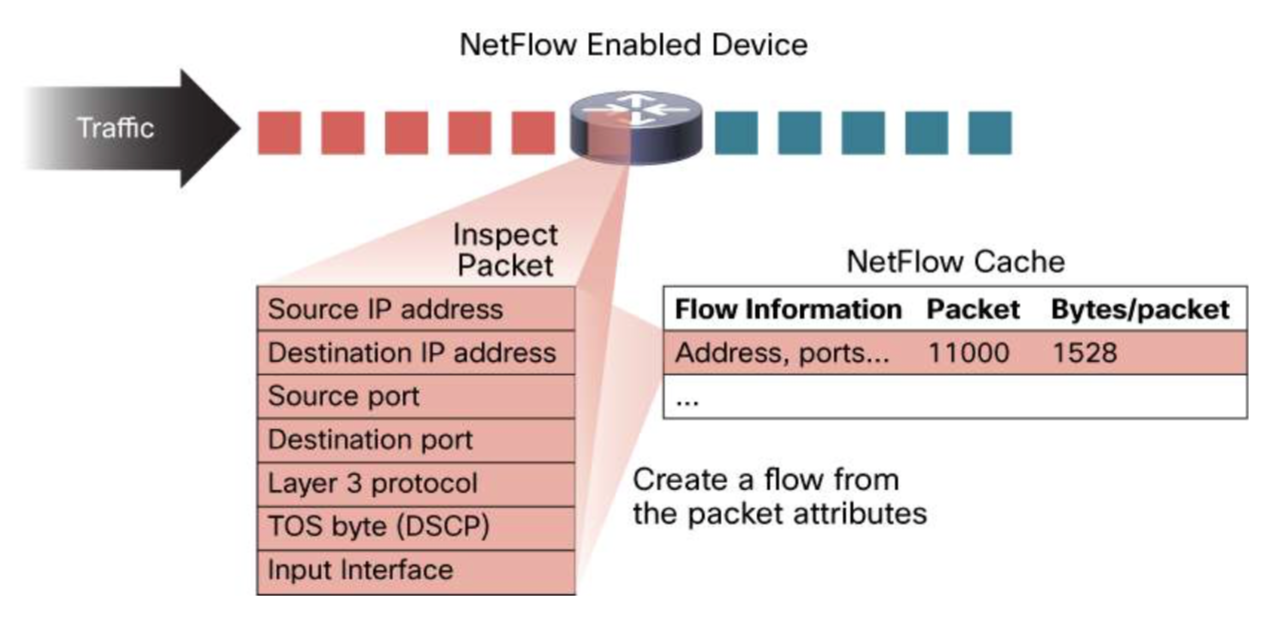
\includegraphics[scale=0.2]{netflow_cache}

\subsection{Main components}
A typical setup using NetFlow consists of three main components:

\begin{itemize}
\item \textbf{Flow Exporter:} aggregates packets into flows and exports flow records towards one or more flow collectors. 

\item \textbf{Flow collector:} is responsible for reception, storage and pre-processing of flow data received from a flow exporter.

\item \textbf{Analysis application:} an application that analyze the received flow data in different contexts, such as intrusion or traffic profiling.
\end{itemize}

\section{Data visualization}
Data visualization refers to the techniques used to communicate data or information by encoding it as visual objects[sitere?]. Meaning that information is represented trough any visual element such as graphs and plots, but may also take any other visual form. Visualization helps users analyse and interact with data in a whole new way. It makes complex data more accessible, understandable and usable. 

In recent years the rate of which data is generated has increased rapidly, and the need for information to be available and comprehensible is growing. All these new sources of data has created what we refer to as "Big Data". Without visual presentation such data is too big to understand. This is the big reason for visualization is emerging as a big market. 

Combining several parameters through visualization could reveal something automated systems might ignore or don't pick up on. "The greatest value of a picture is when it forces us to notice what we never expected to see."[kilde på wiki] by John Tukey.

\subsection{Characteristics}
In his 1983 book The Visual Display of Quantitative Information, Edward Tufte defines characteristics any effective graphical representation should contain as:

\begin{itemize}
\item show the data
\item induce the viewer to think about the substance rather than about methodology, graphic design, the technology of graphic production or something else
\item avoid distorting what the data has to say
\item present many numbers in a small space
\item make large data sets coherent
\item encourage the eye to compare different pieces of data
\item reveal the data at several levels of detail, from a broad overview to the fine structure
\item serve a reasonably clear purpose: description, exploration, tabulation or decoration
\item be closely integrated with the statistical and verbal descriptions of a data set.
\end{itemize}

\subsection{Visual perception}
In this paper the correlation between effective visual communication and how it is perceived upon human inspection is important. A humans ability to distinguish between differences in length, shape and color is referred to as "pre-attentive attributes".  

A good example of this is imagining finding the number of a certain character in a series of characters. This requires significant time and effort, but if the character were to stand out by being a different size, color or orientation this could be done quickly trough pre-attentive processing. Good data visualization takes all of this into consideration and uses pre-attentive processing.
In this simple example it is easy to see how pre attentive processing is used to distinguish how many occurrences of the number 5 is in a larger set of numbers. 
\newline
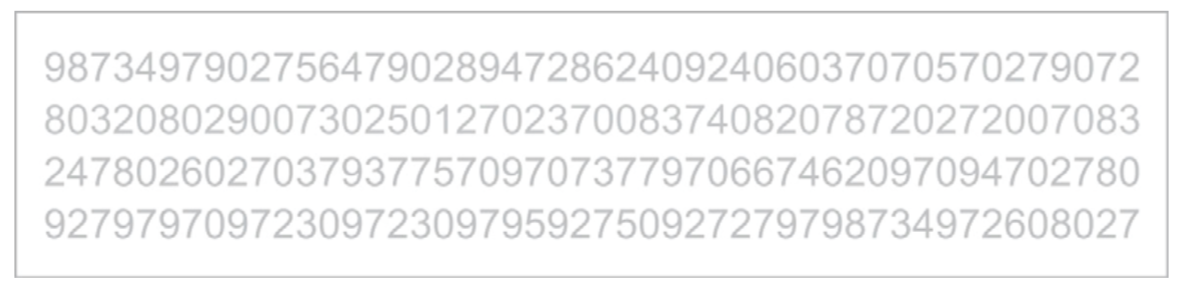
\includegraphics[scale=0.2]{attentive}
\newline
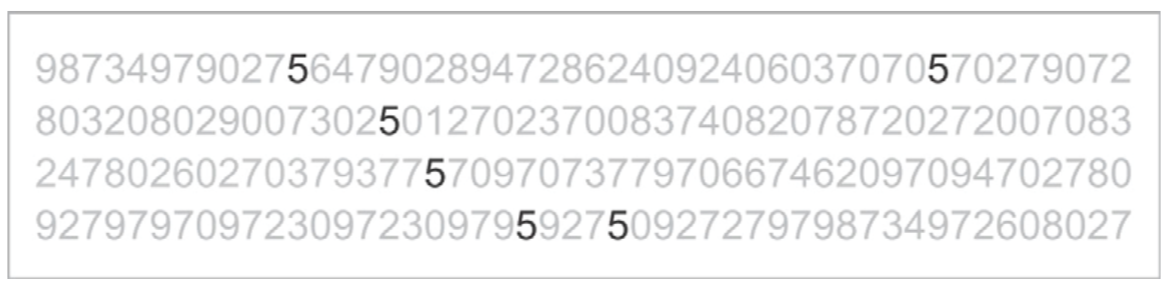
\includegraphics[scale=0.2]{pre_attentive}

\subsection{Data presentation architecture}
Data presentation architecture(DPA) has its purpose to identify, locate, manipulate, format and present data in such a way as to optimally communicate meaning and proffer knowledge[kilde]. This has become an important tool in Business Intelligence, the art of transforming raw data into something useful. 

\subsubsection{Objectives}
DPA has two main objectives, which is the following:

\begin{itemize}
\item To use data to provide knowledge in the most efficient manner possible (minimize noise, complexity, and unnecessary data or detail given each audience's needs and roles)
\item To use data to provide knowledge in the most effective manner possible (provide relevant, timely and complete data to each audience member in a clear and understandable manner that conveys important meaning, is actionable and can affect understanding, behaviour and decisions)
\end{itemize}

\subsubsection{Scope}
The actual work of DPA consist of:
\begin{itemize}
\item Creating effective delivery mechanisms
\item Define relevant knowledge needed by each viewer
\item Determine how often the data should be updated
\item Determine how often and when the user needs to see the data
\item Finding the right data
\item Utilizing the best visualizations and presentation formats
\end{itemize}


\section{D3.js}
In this paper D3.js is chosen as the framework to create examples of effective data visualizations due to its dynamical and interactive properties. 
D3 stands for Data-Driven Documents, and is a Javascript library. It uses widely implemented SVG, CSS and HTML5 standards. D3 is unique in the way it creates SVG objects from large datasets using simple D3.js functions to generate rich text/graphic charts and diagrams. 

